\documentclass{article} \usepackage{amsmath} \usepackage{amssymb} \usepackage{amsthm} \usepackage[margin=0.2in]{geometry} \usepackage{hyperref} \usepackage{physics} \usepackage{tikz} \usepackage{mathtools} \mathtoolsset{showonlyrefs} \theoremstyle{definition} \newtheorem{theorem}{Theorem}[section] \newtheorem{corollary}{Corollary}[theorem] \newtheorem{lemma}[theorem]{Lemma} \newtheorem{definition}{Definition}[section] \author{Connor Duncan} \date{\today}
\title{Physics-105-Lecture-Notes-02-07-2019}
\begin{document}
\maketitle\tableofcontents
\noindent\abstract{A single PDF with all lectures in a single document can be downloaded at \url{https://www.dropbox.com/sh/8sqzvxghvbjifco/AAC9LoSRnsRQDp7pYedgWpQMa?dl=0}. The password is 'analytic.mech.dsp'.
 This file was automatically generated using a script, so there might be some errors. If there are, you can contact me at \url{mailto:ctdunc@berkeley.edu}.}
\section{More Lagrangian Mechanics} \subsection{Pertubations w/ a pendulum} Imagine two pendulums as follows \begin{center} \begin{tikzpicture} \draw (-1,1)--(1,1); \draw (-1,-1)--(1,-1); \draw (0,-1) -- (0,-0.35) ellipse (0.05); \draw (0,1)--(0,0.55) ellipse (0.05); \end{tikzpicture} \end{center} small pertubations will be stable for the top pendulum in gravity, about $\theta=0$, but unstable for the lower. General solution for for $\theta$ at 0 is given as \begin{equation} \delta\theta=A_1e^{-i\omega_0t}+A_2e^{i\omega_0t} \end{equation} if $\theta=\pi$, we find \begin{align} \delta\ddot\theta=\omega_0^2\delta\theta \end{align} which gives \begin{equation} \delta\theta=A_1e^{-\omega_0t}+A_2e^{-\omega_0t} \end{equation} This comes from finding solutions to differential equations. You probably should have taken 54 as a prerequisite to this class, but if u didn't hmu for textbooks (totally legal i promise\footnote{no promises}). \subsection{Interesting thing to do at home} \begin{center} \begin{tikzpicture} \draw (-0.5,0)--(0.5,0); \draw (0,0)--(1,0); \draw (0,0)--(.25,.75); \draw[dashed] (0,0)--(0,1); \draw (.25,.75) ellipse (0.02); \draw[<->](-1,-0.25)--(-1,0.25) node[anchor=west]{$\omega$}; \end{tikzpicture} \end{center} ground is oscillating, with $\omega>>\omega_0$ of the pendulum, \subsection{More general} take some lagrangian \begin{equation} \mathcal{L}=\frac{1}{2}\dot{q}^2-V(q) \end{equation} then equilibrium given by \begin{equation} \pdv{V}{q}=0\rightarrow q=q_0 \end{equation} Take some $q=q_0+\delta q$, then the lagrangian is given \begin{align} && \mathcal{L}=\frac{1}{2}(\delta\dot q)^2-V(q_0+\delta q)= \frac{1}{2}\delta\dot{q}^2-\frac{1}{2}\left(\pdv[2]{V}{q}\right)_{q=q_0}\partial q^2\\ && \partial \ddot q=-\left(\pdv[2]{V}{q}\right)_0\delta q\\ \delta q=Ae^{i\omega t} && \omega^2=\pdv[2]{V}{q}_0\geq 0 \end{align} which gives the sort of intuitive solution that there needs to be a potential well around stable systems, i.e. \begin{center} 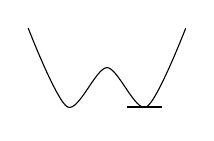
\begin{tikzpicture} \draw plot [smooth] coordinates {(-1,1) (-.5,0) (0,0.5) (.5,0) (1,1)}; \draw (.25,0)--(0.7,0); \end{tikzpicture} \end{center} where the curve represents potential. \subsection{Two Pendulum system} I'm not going to do a drawing of this one. Length of p1 is $l_1$, $l_2$, angle to vertical given by $\theta_n$, where n represents the penulum number, similarly for the mass. We have \begin{align} U=-m_1gl_2\cos\theta_1-m_2g(l_2\cos\theta_1+l_2\cos\theta_2)\\ T=\frac{1}{2}m_1(\dot{x_1}^2+\dot{y_1}^2)+\frac{1}{2}m_2(\dot{x_2}^2+\dot{y_2}^2) \end{align} example for $x_2,y_2$: given by \begin{align} x_2=l_1\sin\theta_1+l_2\sin\theta_2\\ y_2=-l_1\cos\theta_1-l_2\cos\theta_2 \end{align} We get some really really really long for for the lagrangian, which it's almost certainly too long to type. Just do the derivative, and you get that it's \begin{equation} \mathcal L=T-U \end{equation} The solution is then given for \begin{equation} \dv{}{t}\left(\frac{d\mathcal L}{\theta_i}\right)=\pdv{\mathcal{L}}{\theta_i} \end{equation} only equilibrium point is given for $\theta_i=0\forall i$. Even if the pendulums were perpendicular to each other, it would be in unstable equilibrium. Now, we want to linearize the system so that there are only quadratic terms in the lagrangian. No higher powers than 2. for small $\theta$, we just taylor expand everything, gives us \begin{align} \mathcal L=\frac{1}{2}(m_1+m_2)l_2^2\dot{\theta_1}^2+\frac{1}{2}m_2l_2^2\dot{\theta_2}^2\\ +m_2l_1l_2\dot{\theta_1}\dot{\theta_2}+\frac{1}{2}(m_1+m_2)gl_1\theta_1^2+\frac{1}{2}m_2gl_2\theta_2^2 \end{align} We can simplify this down, wiriting \begin{align} \mathcal L=\frac{1}{2}\dot{\theta_1}^2+\frac{1}{2}\mu l^2\dot{\theta_2}^2+\mu l\dot{\theta_1}\dot{\theta_2} -\frac{1}{2}\omega_0^2\theta_1\theta_1^2-\frac{1}{2}\mu l\omega_0^2\theta_2^2 \end{align} with \begin{align} \mu=\frac{m_2}{m_1+m_2} && l=\frac{l_2}{l_1} \end{align} This yields \begin{align} \ddot{\theta_1}+\mu l\ddot{\theta_2}=-\omega_2^2\theta_1\\ l\ddot{\theta_2}+\ddot{\theta_1}=-\omega_0^2\theta_2 \end{align} Now, we rewrite in matrix form, trying to find $\theta_i=A_ie^{i\omega t}$. \begin{equation} \begin{bmatrix} \omega_0^2-\omega^2 & -\mu l\omega^2\\ -\omega^2 & \omega_0^2-\omega^2l \end{bmatrix} \begin{bmatrix}A_1\\A_2\end{bmatrix}=0 \end{equation} Let's call that matrix $D$, and take it's determinant, to see if either $A_1,A_2$ must be zero. \begin{equation} ||D||=(1-\mu)l\omega^4-\omega^2\omega_0^2(1+l)+\omega_0^4 \end{equation} The solutions then, are given as \begin{equation} \omega_\pm^2=\frac{\omega_0^2(1-l)\pm\sqrt{(1+l)^2-4(1-\mu)l}}{2(1-\mu)l} \end{equation} Now, we consider $A_-,A_+$, then, we can write \begin{equation} \theta_y=C_y^+A_y^+e^{i\omega_+t}+C_y^-A_y^-e^{i\omega_-t} \end{equation} with $C_i$ as the initial condition. \begin{enumerate} \item Equilibrium \item Linearize \item $\omega\rightarrow A_i$ \item something else \end{enumerate} These represent the normal modes of a system. Lets consider the equation with the matrix $D$ for the case of $\omega_+$. It's provable that $\omega_+^2>\omega_0^2$, so we take \begin{align} && (\omega_0^2-\omega_+^2)A_1=\mu l\omega_+^2A_2\\ A_1=\frac{\mu l\omega_+^2}{\omega_0^2-\omega_+^2}A_2 && \operatorname{sign}\frac{A_1}{A_2}=-1 \end{align} \subsection{Four points on circle} Take four points on a circle, all of which are connected by springs of coefficient $k$. (I might add a drawing of this later, it's kind of hard to picture). All points are of the same mass. \begin{align} \mathcal L=\frac{1}{2}mR^2\sum_{i=1}^4\dot{\varphi_i}^2-\\ \frac{1}{2}k\times R^2\left[(\varphi_1-\varphi_2)^2+(\varphi_1-\varphi_4)^2+(\varphi_2-\varphi_3)^2+(\varphi_2-\varphi_4)^2\right] \end{align} Which gives a bunch of coupled oscillatros, for $\ddot\varphi _i$. It's more convenient to write them as a giant matrix \begin{equation} \begin{bmatrix} 2\omega_0^2-\omega^2 & -\omega_0^2 & 0 & -\omega_0^2\\ -\omega_0^2 & 2\omega_0^2-\omega^2 & -\omega_0^2 & 0\\ 0 & -\omega_0^2 & -2\omega_0^2-\omega^2 -\omega_0^2 \\ -\omega_0^2 & 0 & -\omega_0^2 & 2\omega_0^2-\omega^2 \end{bmatrix} \begin{bmatrix} A_1\\A_2\\A_3\\A_4 \end{bmatrix}=0 \end{equation} We compute the determinant, and find that \begin{equation} ||D||=\pm(2\omega_0^2-\omega^2)(4\omega_0^2-\omega^2)\omega^2=0 \end{equation} There are some eigenmodes, \begin{align} \omega=0 && \omega=2\omega_0 && \omega=\sqrt{2}\omega_0 \end{align}
\end{document}
